\documentclass[tikz,border=5pt]{standalone}
\usepackage{tikz}\n\usepackage{amssymb}
\usetikzlibrary{shapes.geometric, arrows.meta, positioning, calc, backgrounds, matrix, fit}
\definecolor{pbblue}{HTML}{E6F3FF}
\definecolor{pbdarkblue}{HTML}{1E3A8A}
\definecolor{pbmint}{HTML}{E0F2F1}
\definecolor{pbdarkgreen}{HTML}{065F46}
\definecolor{pbcoral}{HTML}{FEE2E2}
\definecolor{pbdarkred}{HTML}{991B1B}
\definecolor{pbgray}{HTML}{F3F4F6}

\begin{document}
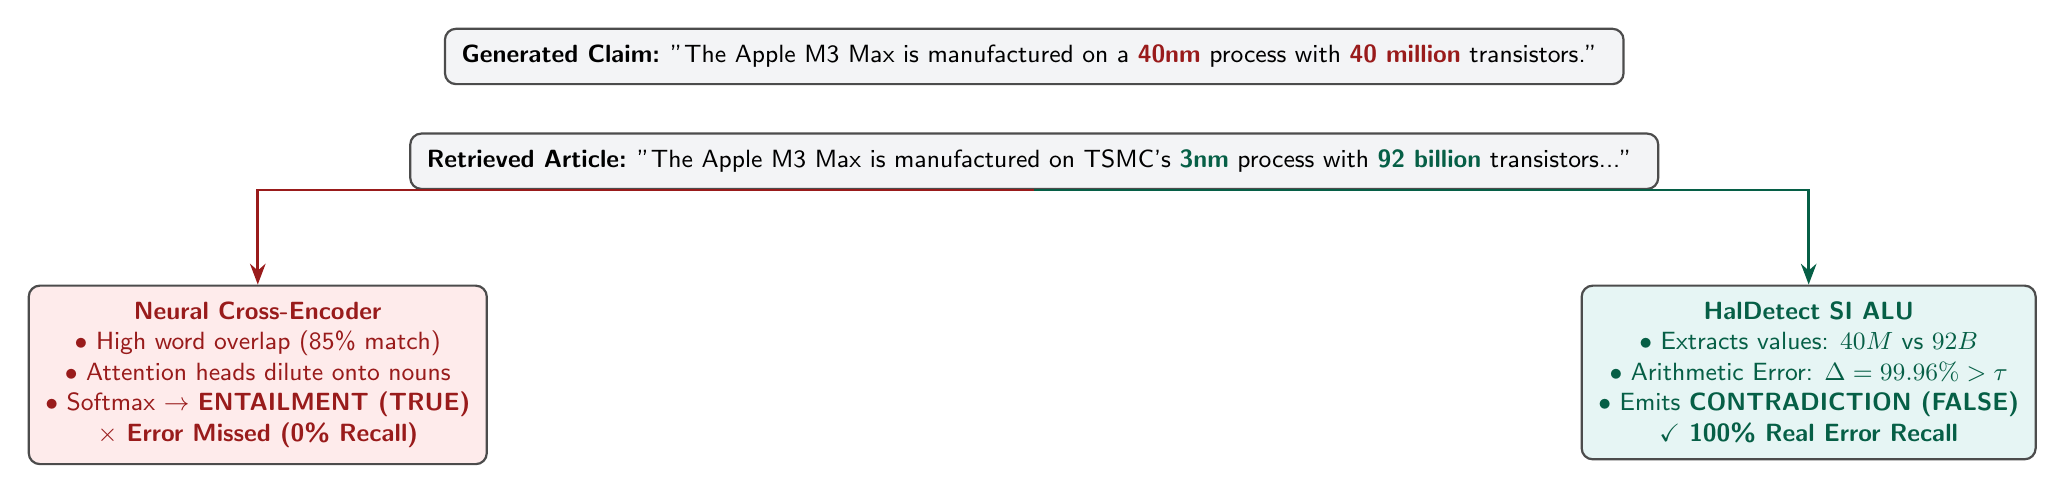
\begin{tikzpicture}[
    font=\sffamily\small,
    box/.style={draw=black!70, rounded corners=4pt, line width=0.8pt, align=center, inner sep=6pt},
    arrow/.style={-{Stealth[scale=1.0]}, line width=1pt, draw=black!70}
]

% Claim box
\node[box, fill=pbgray, minimum width=10cm, align=left] (claim) {
    \textbf{Generated Claim:} "The Apple M3 Max is manufactured on a \textcolor{pbdarkred}{\textbf{40nm}} process with \textcolor{pbdarkred}{\textbf{40 million}} transistors."
};

% Retrieved Passage box
\node[box, fill=pbgray, below=0.6cm of claim, minimum width=10cm, align=left] (passage) {
    \textbf{Retrieved Article:} "The Apple M3 Max is manufactured on TSMC's \textcolor{pbdarkgreen}{\textbf{3nm}} process with \textcolor{pbdarkgreen}{\textbf{92 billion}} transistors..."
};

% Neural RAG Path (Left)
\node[box, fill=pbcoral!70, text=pbdarkred, below left=1.2cm and -1.0cm of passage, minimum width=4.5cm] (neural) {
    \textbf{Neural Cross-Encoder}\\
    $\bullet$ High word overlap (85\% match)\\
    $\bullet$ Attention heads dilute onto nouns\\
    $\bullet$ Softmax $\rightarrow$ \textbf{ENTAILMENT (TRUE)}\\
    \textbf{$\times$ Error Missed (0\% Recall)}
};

% HalDetect ALU Path (Right)
\node[box, fill=pbmint!80, text=pbdarkgreen, below right=1.2cm and -1.0cm of passage, minimum width=4.5cm] (alu) {
    \textbf{HalDetect SI ALU}\\
    $\bullet$ Extracts values: $40\text{M}$ vs $92\text{B}$\\
    $\bullet$ Arithmetic Error: $\Delta = 99.96\% > \tau$\\
    $\bullet$ Emits \textbf{CONTRADICTION (FALSE)}\\
    \textbf{$\checkmark$ 100\% Real Error Recall}
};

\draw[arrow, draw=pbdarkred] (passage.south) -| (neural.north);
\draw[arrow, draw=pbdarkgreen] (passage.south) -| (alu.north);

\end{tikzpicture}
\end{document}